\documentclass[conference]{IEEEtran}
\IEEEoverridecommandlockouts

\usepackage{cite}
\usepackage{amsmath,amssymb,amsfonts}
\usepackage{graphicx}
\usepackage{textcomp}
\usepackage{xcolor}
\usepackage{booktabs}
\usepackage{url}
\usepackage{tikz}
\usetikzlibrary{shapes.geometric, arrows, positioning, fit, calc}

\def\BibTeX{{\rm B\kern-.05em{\sc i\kern-.025em b}\kern-.08em
    T\kern-.1667em\lower.7ex\hbox{E}\kern-.125emX}}

\begin{document}

\title{Drishti-Kavach: Advancing India's Railway Security System with Spatial Clearance Perception Engine for Next-Generation Railway Safety}

\author{
    \setlength{\tabcolsep}{24pt}
    \begin{tabular}{cc}
        \textbf{Gowri Krishnan Nair} & \textbf{Ananya Sanjiv} \\
        \textit{Dept. of CSE} & \textit{Dept. of CSE} \\
        \textit{MVJ College of Engineering} & \textit{MVJ College of Engineering} \\
        Bengaluru, India & Bengaluru, India \\
        1mj23cs061@mvjce.edu.in & 1mj23cs015@mvjce.edu.in \\[0.45cm]
    \end{tabular}
    \\
    \setlength{\tabcolsep}{16pt}
    \begin{tabular}{ccc}
        \textbf{Alvin Sonny} & \textbf{Ganesha Thejaswi V} & \textbf{KL Sujitha} \\
        \textit{Dept. of CSE} & \textit{Dept. of CSE} & \textit{Dept. of CSE} \\
        \textit{MVJ College of Engineering} & \textit{MVJ College of Engineering} & \textit{MVJ College of Engineering} \\
        Bengaluru, India & Bengaluru, India & Bengaluru, India \\
        1mj23cs012@mvjce.edu.in & 1mj23cs058@mvjce.edu.in & slakkaiyan@gmail.com \\
    \end{tabular}
}

\maketitle

\begin{abstract}
Traditional railway safety mechanisms---including fixed block track circuits, axle counters, and transponder-based Train Collision Avoidance Systems (TCAS / Kavach)---rely strictly on block-occupancy signals and cab-signaling telemetry. While effective against train-to-train collisions, these systems lack forward optical perception and are fundamentally blind to non-signaled track intrusions, level-crossing vehicular blockades, fallen trees, landslides, and deliberate track sabotage (e.g., steel rods, placed rail sections, and flammable canisters). In this paper, we present \textbf{Drishti-Kavach}, an edge-deployable, dual-spectrum optical Automatic Train Protection (ATP) perception engine engineered for real-time locomotive forward lookahead. Drishti-Kavach decouples visual perception into a lightweight bilateral semantic segmentation network (\textbf{BiSeNetV2}, $\sim$3.49M parameters) for drivable ballast gauge and steel rail ribbon extraction, paired with a high-resolution ($1024\times1024$) \textbf{YOLO11m} detector for micro-sabotage and physical hazard localization. To resolve 24/7 environmental degradation, an atmospheric optical enhancer dynamically couples Dark Channel Prior (DCP) transmission estimation with Luminance-domain CLAHE, operating in tandem with an active 850nm Near-Infrared (NIR) headlamp modeling framework. Rather than employing black-box collision classification, a deterministic \textbf{Vector Spatial Clearance Engine} applies Shapely polygon unions, base ground footprint projections, and dynamic lateral safety buffering to classify threats into a 3-tier hierarchy (CRITICAL, WARNING, CLEAR). Evaluated across a multimodal benchmark combining RailSem19 and Indian UAV-RSOD datasets, Drishti-Kavach achieves \textbf{86.02\% Universal mIoU} (90.08\% Track Bed IoU) and \textbf{90.90\% AP@50} on deliberate track sabotage (\textit{IronRod}), while operating at \textbf{$>$50 FPS} on edge accelerators with sub-20ms total latency.
\end{abstract}

\begin{IEEEkeywords}
Automatic Train Protection (ATP), Intelligent Transportation Systems (ITS), Semantic Segmentation, Obstacle Detection, BiSeNetV2, YOLO11m, Active Near-Infrared Vision, Spatial Clearance Geometry, Railway Sabotage Prevention.
\end{IEEEkeywords}

\section{Introduction}

Modern railway networks represent the critical infrastructure backbone of national economies. On high-density rail corridors such as the Indian Railways network, safety has historically depended on automated signaling infrastructures, fixed block circuits, and radio-frequency transponders such as \textbf{Kavach (TCAS - Train Collision Avoidance System)}. While Kavach enforces Signal Passed at Danger (SPAD) prevention and locomotive-to-locomotive head-on collision avoidance, recent surveys on railway safety \cite{xu2025advancements, chen2025realtime} underscore an intrinsic structural limitation: \textit{conventional transponders cannot perceive physical track blockades ahead of the train}.

Physical derailments and catastrophic railway collisions frequently occur due to un-signaled obstructions lying outside the capability envelope of track circuits \cite{xu2025advancements}:
\begin{enumerate}
    \item \textbf{Deliberate Sabotage:} Foreign steel girders, severed rail pieces, or fishplates placed across running rails to induce derailment.
    \item \textbf{Level-Crossing Gate Entrapment:} Passenger road vehicles, trucks, and buses stalled within the railway clearance envelope.
    \item \textbf{Geological and Washout Hazards:} Boulders from mountain rockfalls, washed-out ballast, and storm-felled tree limbs.
    \item \textbf{Human and Wildlife Trespassing:} Track maintenance gangs, pedestrians, and livestock crossing blind curves.
    \item \textbf{Atmospheric Blindness:} Severe winter radiation fog, monsoon precipitation, and night darkness that impair locomotive drivers' vision beyond safe emergency braking distances.
\end{enumerate}

To bridge this critical safety gap, we introduce \textbf{Drishti-Kavach}, an optical Automatic Train Protection perception engine. Our primary technical contributions are:
\begin{itemize}
    \item \textbf{Decoupled Dual-Engine Architecture:} We eliminate gradient conflict between dense boundary segmentation and small-object detection by separating track bed parsing (BiSeNetV2) from micro-sabotage detection (YOLO11m at $1024\times1024$).
    \item \textbf{Universal Dual Training Protocol:} We introduce a multimodal dataset synthesis strategy integrating first-person locomotive cab feeds (RailSem19) with aerial/infrastructure feeds (UAV-RSOD V1), regularized with physics-based Active 850nm NIR Night Vision synthesis to prevent catastrophic forgetting.
    \item \textbf{Deterministic Vector Spatial Clearance Engine:} Moving away from brittle black-box classifiers, we employ Shapely vector polygon geometry, bottom 25\% ground footprint projection, and dynamic lateral buffers ($\delta=65\text{px}$) to compute verifiable ATP intervention triggers.
    \item \textbf{Atmospheric Optical Enhancer:} An adaptive multi-mode module that scores atmospheric fog density via Dark Channel Prior (DCP) statistics and executes localized LAB Luminance CLAHE for haze and monsoon rain suppression.
\end{itemize}

\begin{figure*}[!t]
\centering
\resizebox{0.96\textwidth}{!}{
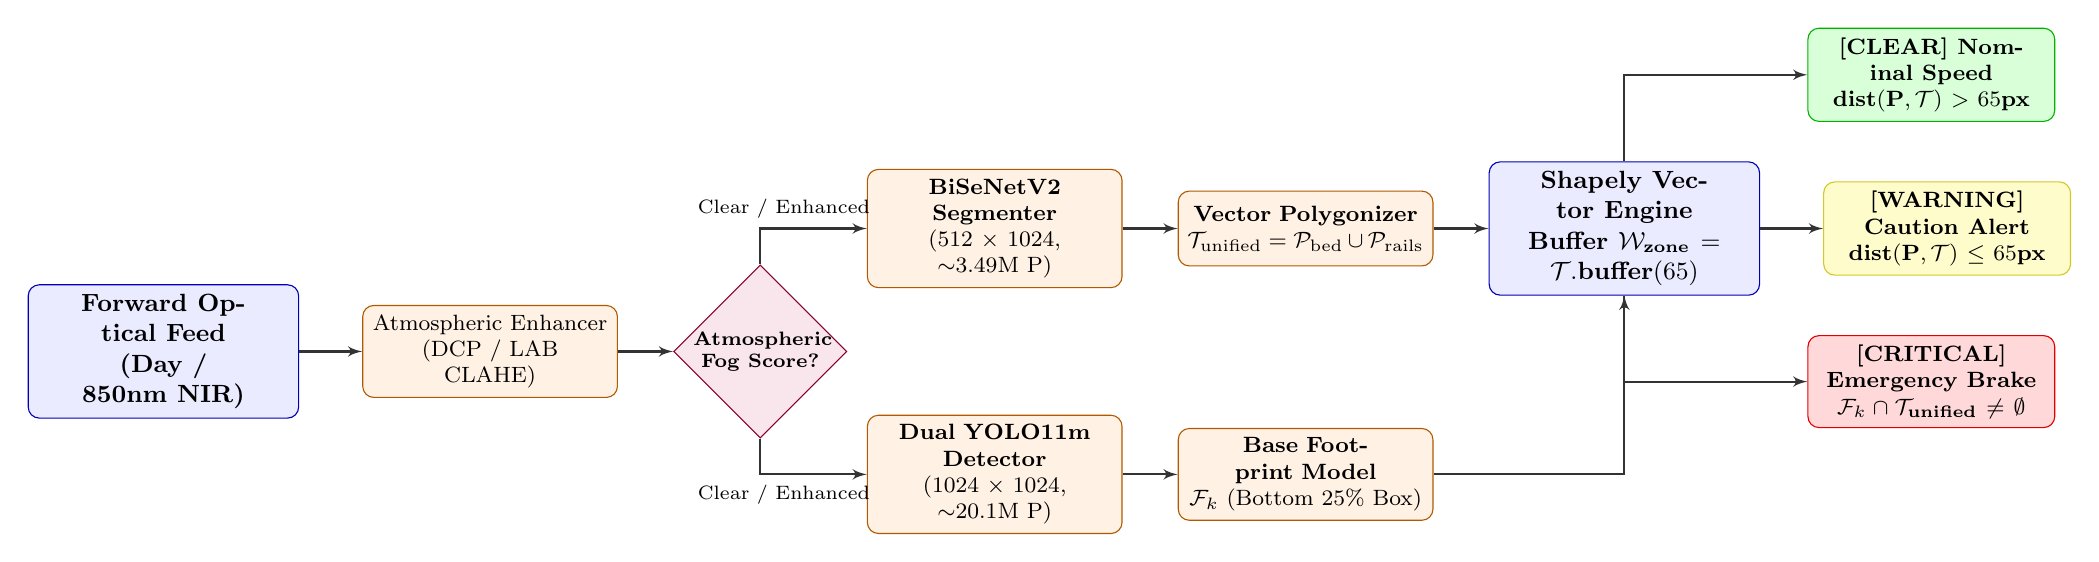
\begin{tikzpicture}[
    node distance=0.9cm and 0.6cm,
    block/.style={rectangle, draw=blue!70!black, fill=blue!8, rounded corners=4pt, text width=3.2cm, text centered, minimum height=1.0cm, font=\small\bfseries},
    proc/.style={rectangle, draw=orange!70!black, fill=orange!10, rounded corners=4pt, text width=3.0cm, text centered, minimum height=0.95cm, font=\footnotesize},
    decision/.style={diamond, draw=purple!70!black, fill=purple!10, text width=1.7cm, text centered, inner sep=0pt, font=\scriptsize\bfseries},
    output_crit/.style={rectangle, draw=red!90!black, fill=red!15, rounded corners=4pt, text width=2.9cm, text centered, minimum height=0.95cm, font=\footnotesize\bfseries},
    output_warn/.style={rectangle, draw=yellow!80!black, fill=yellow!20, rounded corners=4pt, text width=2.9cm, text centered, minimum height=0.95cm, font=\footnotesize\bfseries},
    output_safe/.style={rectangle, draw=green!70!black, fill=green!15, rounded corners=4pt, text width=2.9cm, text centered, minimum height=0.95cm, font=\footnotesize\bfseries},
    line/.style={draw=black!80, -latex', thick}
]

% Top Row: Input -> Optics -> Decision
\node [block] (input) {Forward Optical Feed\\(Day / 850nm NIR)};
\node [proc, right=0.8cm of input] (optics) {Atmospheric Enhancer\\(DCP / LAB CLAHE)};
\node [decision, right=0.7cm of optics] (fogchk) {Atmospheric\\Fog Score?};

% Parallel Engines
\node [proc, above right=0.25cm and 0.8cm of fogchk] (seg) {\textbf{BiSeNetV2 Segmenter}\\($512\times1024$, $\sim$3.49M P)};
\node [proc, below right=0.25cm and 0.8cm of fogchk] (det) {\textbf{Dual YOLO11m Detector}\\($1024\times1024$, $\sim$20.1M P)};

% Geometric Conversion
\node [proc, right=0.7cm of seg] (poly) {\textbf{Vector Polygonizer}\\$\mathcal{T}_{\text{unified}} = \mathcal{P}_{\text{bed}} \cup \mathcal{P}_{\text{rails}}$};
\node [proc, right=0.7cm of det] (foot) {\textbf{Base Footprint Model}\\$\mathcal{F}_k$ (Bottom 25\% Box)};

% Spatial Reasoning Engine
\node [block, right=0.7cm of poly] (hazard) {Shapely Vector Engine\\Buffer $\mathcal{W}_{\text{zone}} = \mathcal{T}.\text{buffer}(65)$};

% 3-Tier Threat Outputs
\node [output_safe, above right=0.5cm and 0.6cm of hazard] (clear) {[CLEAR] Nominal Speed\\$\text{dist}(\mathbf{P}, \mathcal{T}) > 65\text{px}$};
\node [output_warn, right=0.8cm of hazard] (warning) {[WARNING] Caution Alert\\$\text{dist}(\mathbf{P}, \mathcal{T}) \le 65\text{px}$};
\node [output_crit, below right=0.5cm and 0.6cm of hazard] (crit) {[CRITICAL] Emergency Brake\\$\mathcal{F}_k \cap \mathcal{T}_{\text{unified}} \neq \emptyset$};

% Connections
\path [line] (input) -- (optics);
\path [line] (optics) -- (fogchk);
\path [line] (fogchk) |- node[above, font=\scriptsize, xshift=0.3cm]{Clear / Enhanced} (seg);
\path [line] (fogchk) |- node[below, font=\scriptsize, xshift=0.3cm]{Clear / Enhanced} (det);
\path [line] (seg) -- (poly);
\path [line] (det) -- (foot);
\path [line] (poly) -- (hazard);
\path [line] (foot) -| (hazard);
\path [line] (hazard) |- (clear);
\path [line] (hazard) -- (warning);
\path [line] (hazard) |- (crit);

\end{tikzpicture}
}
\caption{End-to-End Functional Architecture Flowchart of the Drishti-Kavach Decoupled Optical Automatic Train Protection Engine.}
\label{fig:pipeline_flowchart}
\end{figure*}

\section{Related Work}

\subsection{Railway Intrusion Detection \& Perception Frameworks}
Comprehensive reviews by Xu \textit{et al.} \cite{xu2025advancements} emphasize that vision-based onboard obstacle intrusion detection systems (OIDSs) are paramount for autonomous train safety. While early research relied on stationary trackside surveillance, onboard vision enables continuous corridor coverage. Chen \textit{et al.} \cite{chen2025realtime} proposed multitask perception learning for real-time obstacle detection across railway sectors, demonstrating that multi-task pipelines must maintain rigorous real-time performance without catastrophic accuracy loss.

\subsection{Deep Learning for Railway Obstacle and Sabotage Detection}
To overcome the limitations of general object detectors on railway tracks, Wang and Du \cite{wang2024yolorail} introduced \textbf{YOLO-Rail}, utilizing ConvNeXtV2 and feature fusion to detect obstacles on rails. Li \textit{et al.} \cite{li2025improved} proposed an improved RT-DETR framework tailored for railway obstacle detection, demonstrating the power of real-time transformer backbones. Eisentraut \textit{et al.} \cite{eisentraut2025leveraging} investigated domain-specific feature extraction for railway obstacle classification, proving that localized physical context is essential to prevent false alarms. In 3D point cloud perception, Lian \textit{et al.} \cite{lian2025rae3d} introduced RAE3D, while Liu \textit{et al.} \cite{liu2025railbev} introduced RailBEV for bird's-eye-view representation.

\subsection{Semantic Track Segmentation and Clearance Geometry}
Accurate delineation of running rails and drivable ballast is required to define the train clearance envelope. Song \textit{et al.} \cite{song2025deep} proposed attention-aggregated semantic segmentation for foreign object intrusion, showing that high-precision boundary extraction reduces spatial ambiguity. Guo \textit{et al.} \cite{guo2026track2net} introduced \textbf{Track2Net}, a fast lightweight keypoint alignment model for rail line tracking. In dynamic clearance modeling, Wu and Li \cite{wu2025research} demonstrated multi-sensor dynamic obstacle avoidance and path clearance reasoning.

\section{System Architecture \& Methodology}

The overall architecture of Drishti-Kavach is illustrated in Fig.~\ref{fig:pipeline_flowchart}.

\subsection{Multi-Spectral Active 850nm Near-Infrared (NIR) Modeling}
To guarantee 24/7 operational capability, we model the physics of locomotive-mounted active 850nm infrared illuminators. The synthetic NIR conversion pipeline applies spectral CMOS sensitivity weighting, conical spotlight attenuation, tone-mapping, and sensor noise:
\begin{equation}
\text{Mono}(x,y) = 0.18 B(x,y) + 0.47 G(x,y) + 0.35 R(x,y)
\end{equation}

The conical illuminator is modeled with radial intensity decay centered at the track vanishing axis $(x_0 = W/2, y_0 = 0.60 H)$:
\begin{equation}
d^2(x,y) = \frac{(x - x_0)^2}{(0.58 W)^2} + \frac{(y - y_0)^2}{(0.48 H)^2}
\end{equation}
\begin{equation}
I_{\text{spot}}(x,y) = \exp\left(-1.4 \cdot d^2(x,y)\right)
\end{equation}
\begin{equation}
I_{\text{NIR}}(x,y) = 0.12 + 0.88 \cdot I_{\text{spot}}(x,y)
\end{equation}
\begin{align}
\text{Frame}_{\text{NIR}}(x,y) = \text{clip}\Big( &\left(\frac{\text{Mono} \cdot I_{\text{NIR}}}{255}\right)^{1.15} \cdot 255 \notag \\
&+ \mathcal{N}(0, 6.0), 0, 255 \Big)
\end{align}

\subsection{Atmospheric Optical Enhancer}
The optical enhancement module monitors atmospheric transmission in real time. It computes an \textbf{Airlight Fog Density Score} $S_{\text{fog}} \in [0, 1]$ combining luminance standard deviation $\sigma_{\text{gray}}$ and dark channel intensity $\mu_{\text{dark}}$:
\begin{equation}
S_{\text{contrast}} = \text{clip}\left(\frac{55.0 - \sigma_{\text{gray}}}{40.0}, 0, 1\right)
\end{equation}
\begin{equation}
S_{\text{airlight}} = \text{clip}\left(\frac{\mu_{\text{dark}} - 60.0}{100.0}, 0, 1\right)
\end{equation}
\begin{equation}
S_{\text{fog}} = 0.60 \cdot S_{\text{airlight}} + 0.40 \cdot S_{\text{contrast}}
\end{equation}

When $S_{\text{fog}} > 0.60$, the system executes Dark Channel Prior (DCP) inversion:
\begin{equation}
J(x) = \frac{I(x) - A}{\max(t(x), t_0)} + A
\end{equation}
When $0.40 < S_{\text{fog}} \le 0.60$, it applies Luminance CLAHE in the LAB color space with clip limit $3.0$ and grid size $(8, 8)$.

\subsection{Track Bed \& Rail Ribbon Segmenter: BiSeNetV2}
BiSeNetV2 handles high-speed semantic track segmentation across three canonical classes: \textit{0: Background}, \textit{1: Track\_Bed}, and \textit{2: Rail\_Lines} \cite{song2025deep, guo2026track2net}.
\begin{enumerate}
    \item \textbf{Detail Branch (Spatial Pathway):} Uses 3 stages of shallow convolutions down to $1/8\times$ scale with 128 feature channels to retain sharp rail boundaries and ballast textures.
    \item \textbf{Semantic Branch (Context Pathway):} Employs a \textit{StemBlock} ($1/4\times$) and Gather-and-Expansion (\textit{GELayer}, $e=6$) inverted bottleneck blocks down to $1/32\times$, terminated by a Context Embedding block (\textit{CEBlock}) with Global Average Pooling (GAP).
    \item \textbf{Bilateral Guided Aggregation (BGA):} Fuses spatial details and semantic cues via bidirectional depthwise separable attention gates:
    \begin{equation}
    \text{Path}_1 = \text{Detail}_{\text{DW}} \odot \sigma(\text{Semantic}_{\text{Up}})
    \end{equation}
    \begin{equation}
    \text{Path}_2 = \text{Interp}\left(\text{Semantic}_{\text{Conv}} \odot \sigma(\text{Detail}_{\text{Down}})\right)
    \end{equation}
    \begin{equation}
    \text{Output}_{\text{BGA}} = \text{Conv}_{3\times3}\left(\text{Path}_1 + \text{Path}_2\right)
    \end{equation}
    \item \textbf{Booster Training vs. Zero-Cost Inference:} 4 auxiliary booster heads inject intermediate supervision gradients during training. These heads are pruned prior to ONNX export, ensuring \textbf{0 FLOPs overhead} at runtime ($\sim$3.49M parameters, 13.3 MB binary).
\end{enumerate}

\subsection{Dual-Layer Railway Sabotage \& Obstacle Detector}
Operating natively at $1024\times1024$ resolution, the detection subsystem runs two cooperating layers \cite{chen2025realtime, wang2024yolorail}:
\begin{itemize}
    \item \textbf{Layer 1 (Custom 8-Class Railway Hazard Engine):} Fine-tuned specifically for \textit{Person}, \textit{Car}, \textit{Truck}, \textit{Branch}, \textit{IronRod}, \textit{Boulder}, \textit{Barrel}, and \textit{Jerrycan}. Trains and locomotives are strictly excluded to prevent false triggers from parallel line traffic.
    \item \textbf{Layer 2 (Complementary Foundation Baseline):} Incorporates 19 enabled COCO foundation classes covering livestock/wildlife, auxiliary transport, and unattended luggage.
    \item \textbf{IoU-Based Fusion:} Merges predictions using non-maximum suppression ($\text{IoU}_{\text{thresh}} = 0.45$), where custom sabotage detections take operational precedence.
\end{itemize}

\section{Vector Spatial Clearance \& ATP Hazard Engine}

Perception bounding boxes and raster masks cannot directly command train braking without spatial context. Drishti-Kavach translates 2D bounding boxes and segmented masks into mathematical vector geometry via the Shapely engine \cite{wu2025research, liu2025railbev}.

\subsection{Bottom 25\% Ground Contact Footprint Model}
To eliminate false overlaps caused by perspective distortion (where an object's head or upper profile projects onto distant background tracks), we model the physical ground contact footprint $\mathcal{F}_k$:
\begin{equation}
\mathcal{B}_k = [x_1, y_1, x_2, y_2], \quad h_k = y_2 - y_1
\end{equation}
\begin{equation}
y_{\text{foot}} = y_2 - 0.25 \cdot h_k
\end{equation}
\begin{equation}
\mathcal{F}_k = \text{Polygon}\big([(x_1, y_{\text{foot}}), (x_2, y_{\text{foot}}), (x_2, y_2), (x_1, y_2)]\big)
\end{equation}
\begin{equation}
\mathbf{P}_{\text{anchor}} = \left(\frac{x_1 + x_2}{2}, y_2\right)
\end{equation}

\subsection{Unified Track Union \& Dynamic Clearance Buffering}
OpenCV contour extraction polygonizes segmented masks into track bed polygons $\mathcal{P}_{\text{bed}}$ and rail line polygons $\mathcal{P}_{\text{rails}}$. A unary union forms the master reference geometry:
\begin{equation}
\mathcal{T}_{\text{unified}} = \text{unary\_union}\left(\mathcal{P}_{\text{bed}} \cup \mathcal{P}_{\text{rails}}\right)
\end{equation}

A dynamic lateral safety envelope is constructed with dilation parameter $\delta = 65\text{ pixels}$:
\begin{equation}
\mathcal{W}_{\text{zone}} = \mathcal{T}_{\text{unified}}.\text{buffer}(\delta)
\end{equation}

\subsection{Three-Tier Threat Classification (ATP Braking Rules)}
\begin{enumerate}
    \item \textbf{[CRITICAL] Threat (In-Track Obstacle $\rightarrow$ ATP Emergency Brake):}
    \begin{equation}
    \mathcal{F}_k \cap \mathcal{T}_{\text{unified}} \neq \emptyset \quad \lor \quad \mathbf{P}_{\text{anchor}} \in \mathcal{T}_{\text{unified}}
    \end{equation}
    \textit{Action:} Triggers emergency brake line via locomotive TCAS sub-rack interface and paints target bounding box in vivid red.
    \item \textbf{[WARNING] Threat (Near-Track Infringement $\rightarrow$ Driver HUD Caution):}
    \begin{equation}
    \left(\mathcal{F}_k \cap \mathcal{W}_{\text{zone}} \neq \emptyset \lor \mathbf{P}_{\text{anchor}} \in \mathcal{W}_{\text{zone}}\right) \land \mathcal{F}_k \cap \mathcal{T}_{\text{unified}} = \emptyset
    \end{equation}
    \textit{Action:} Computes Euclidean track distance $d_k = \text{dist}(\mathbf{P}_{\text{anchor}}, \mathcal{T}_{\text{unified}}) \le 65\text{px}$ and alerts the driver HUD for speed curtailment.
    \item \textbf{[CLEAR] / SAFE State (Off-Track Object $\rightarrow$ Nominal Line Speed):}
    \begin{equation}
    \text{dist}(\mathbf{P}_{\text{anchor}}, \mathcal{T}_{\text{unified}}) > \delta
    \end{equation}
    \textit{Action:} Validates obstacle clearance (e.g., platform passengers or parallel road vehicles); no brake intervention.
\end{enumerate}

\section{Experimental Setup \& Datasets}

\subsection{Curated Datasets}
\begin{enumerate}
    \item \textbf{\textit{dataset\_seg/}} (RailSem19 Cab View): 8,500 cab-view frames remapped into 3-class canonical format (\textit{Background}, \textit{Track\_Bed}, \textit{Rail\_Lines}) with 50/50 Day/Active NIR Night pairs.
    \item \textbf{\textit{dataset\_uav\_v1/}} (UAV-RSOD Infrastructure): High-angle drone and gantry imagery providing structural angle regularization.
    \item \textbf{\textit{dataset\_det/}} (Unified 8-Class Hazard Dataset): Standardized YOLO bounding boxes combining UAV-RSOD V2 sabotage targets and RailSem19 crossing vehicles.
\end{enumerate}

\begin{table}[h]
\caption{Curated Datasets Specification Summary}
\label{tab:datasets}
\centering
\resizebox{\columnwidth}{!}{
\begin{tabular}{@{}llll@{}}
\toprule
\textbf{Curated Directory} & \textbf{Source Benchmark} & \textbf{Output Format} & \textbf{Target Model} \\ \midrule
\textit{dataset\_seg/} & RailSem19 Cab View & 3-Class 8-bit PNG & BiSeNetV2 \\
\textit{dataset\_uav\_v1/} & UAV-RSOD V1 Infra & 3-Class 8-bit PNG & BiSeNetV2 \\
\textit{dataset\_det/} & UAV-RSOD V2 + RailSem & 8-Class YOLO TXT & YOLO11m \\ \bottomrule
\end{tabular}
}
\end{table}

\subsection{Training Hyperparameters}
\begin{itemize}
    \item \textbf{Universal BiSeNetV2:} Trained using AdamW ($\beta_1=0.9, \beta_2=0.999$, weight decay $1\times 10^{-4}$) with polynomial learning rate schedule (initial LR $5\times 10^{-4}$, power $0.9$) over 40 epochs on dual NVIDIA T4/P100 GPUs.
    \item \textbf{YOLO11m Detector:} Trained at native $1024\times1024$ resolution for 50 epochs using Task-Aligned Assigner (TAL), Mosaic augmentations, and CIoU + DFL loss \cite{wang2024yolorail, eisentraut2025leveraging}.
\end{itemize}

\begin{figure*}[!t]
\centering
\begin{minipage}{0.24\textwidth}
    \centering
    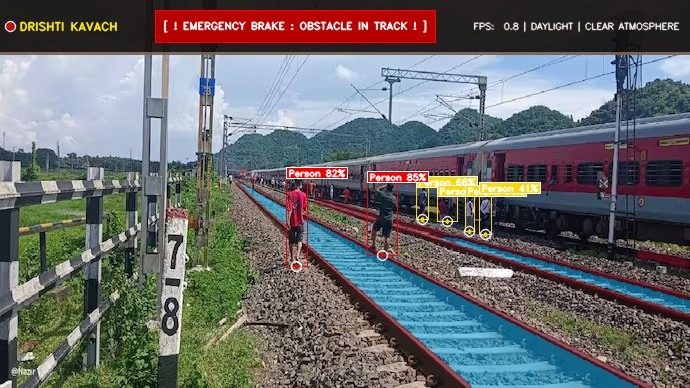
\includegraphics[width=\linewidth]{figures/fig_res1.jpg}
    \centerline{\footnotesize (a) [CRITICAL] Emergency Brake}
    \label{fig:res1}
\end{minipage}\hfill
\begin{minipage}{0.24\textwidth}
    \centering
    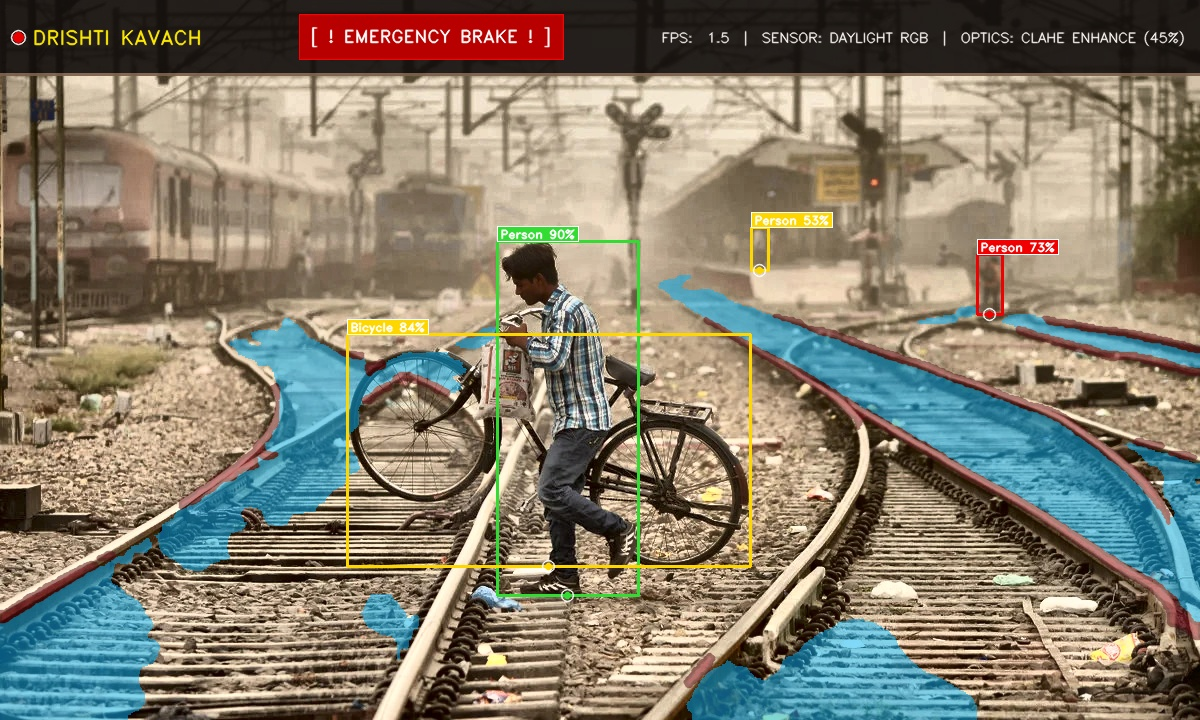
\includegraphics[width=\linewidth]{figures/fig_res2.jpg}
    \centerline{\footnotesize (b) [WARNING] Near-Track Caution}
    \label{fig:res2}
\end{minipage}\hfill
\begin{minipage}{0.24\textwidth}
    \centering
    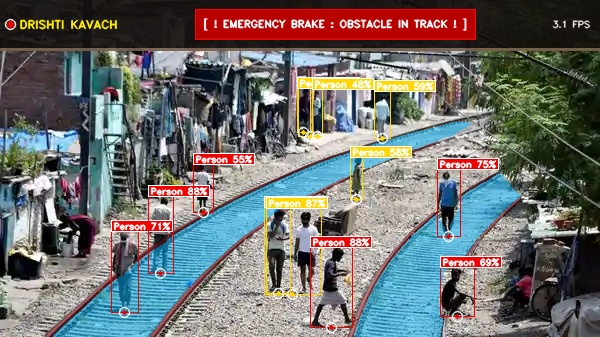
\includegraphics[width=\linewidth]{figures/fig_res3.jpg}
    \centerline{\footnotesize (c) [CLEAR] Platform Clearance}
    \label{fig:res3}
\end{minipage}\hfill
\begin{minipage}{0.24\textwidth}
    \centering
    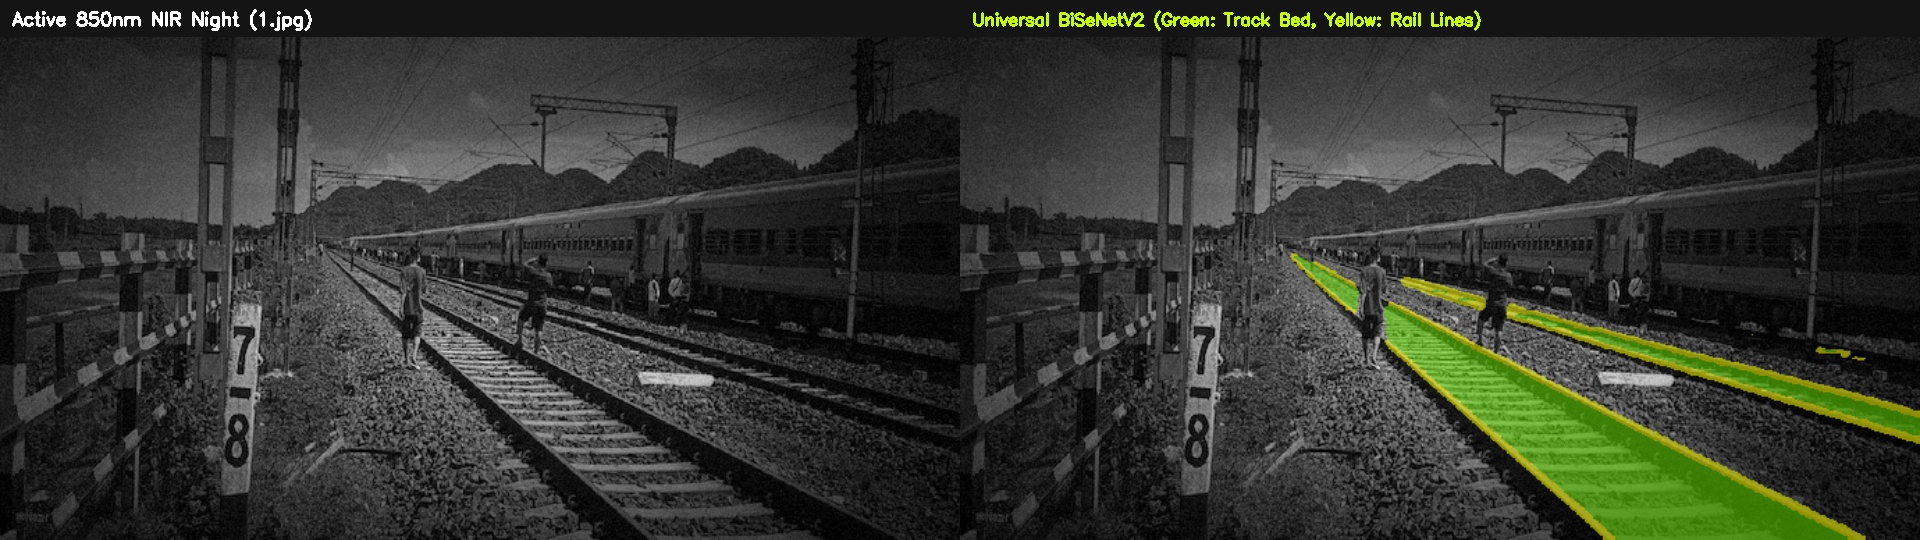
\includegraphics[width=\linewidth]{figures/fig_night1.jpg}
    \centerline{\footnotesize (d) Active 850nm NIR Night Vision}
    \label{fig:daynight}
\end{minipage}
\caption{Qualitative End-to-End Perception, Spatial Clearance Reasoning, and Telemetry HUD Inferences Across Real-World Scenarios.}
\label{fig:results_gallery}
\end{figure*}

\section{Experimental Results \& Benchmarks}

\subsection{Semantic Track Segmentation Performance (Universal BiSeNetV2)}
The segmentation engine achieves \textbf{86.02\% Universal mIoU} and \textbf{98.86\% Pixel Accuracy} across multi-angle validation sets:
\begin{equation}
\text{Mean IoU (mIoU)} = \frac{1}{C}\sum_{c=0}^{C-1} \frac{\text{TP}_c}{\text{TP}_c + \text{FP}_c + \text{FN}_c} = \mathbf{86.02\%}
\end{equation}

\begin{table}[h]
\caption{Semantic Segmentation Performance Breakdown}
\label{tab:seg_metrics}
\centering
\resizebox{\columnwidth}{!}{
\begin{tabular}{@{}lcccc@{}}
\toprule
\textbf{Semantic Class} & \textbf{IoU (\%)} & \textbf{Recall (\%)} & \textbf{Precision (\%)} & \textbf{Dice / F1 (\%)} \\ \midrule
\textbf{Track Bed (Ballast)} & \textbf{90.08} & 94.21 & 95.34 & \textbf{94.78} \\
\textbf{Rail Lines (Rails)} & \textbf{69.11} & 76.50 & 87.80 & \textbf{81.73} \\
\textbf{Background / Sky} & \textbf{98.86} & 99.30 & 99.55 & \textbf{99.43} \\ \midrule
\textbf{Global Summary} & \textbf{86.02} & \textbf{90.00} & \textbf{94.23} & \textbf{91.98} \\ \bottomrule
\end{tabular}
}
\end{table}

\begin{figure}[t]
\centering
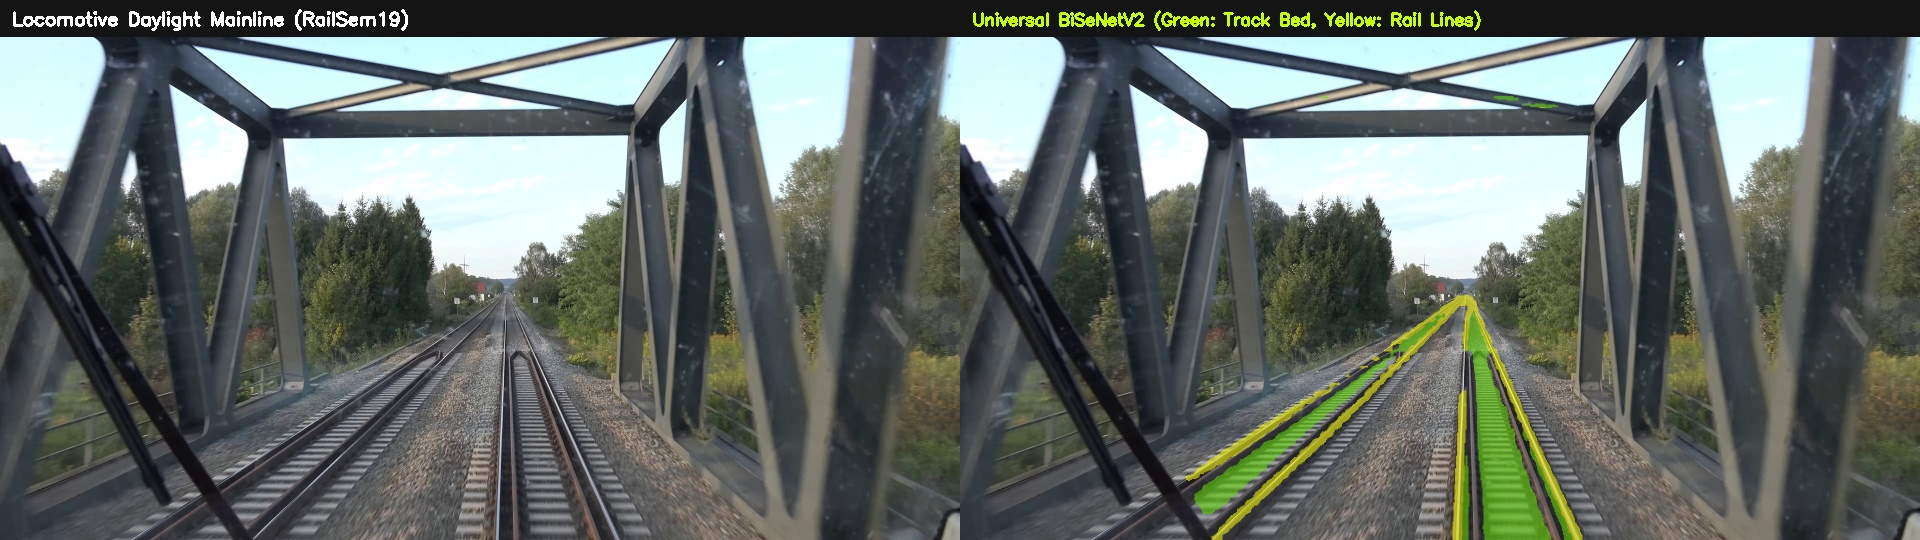
\includegraphics[width=0.48\columnwidth]{figures/fig_universal1.jpg}
\hfill
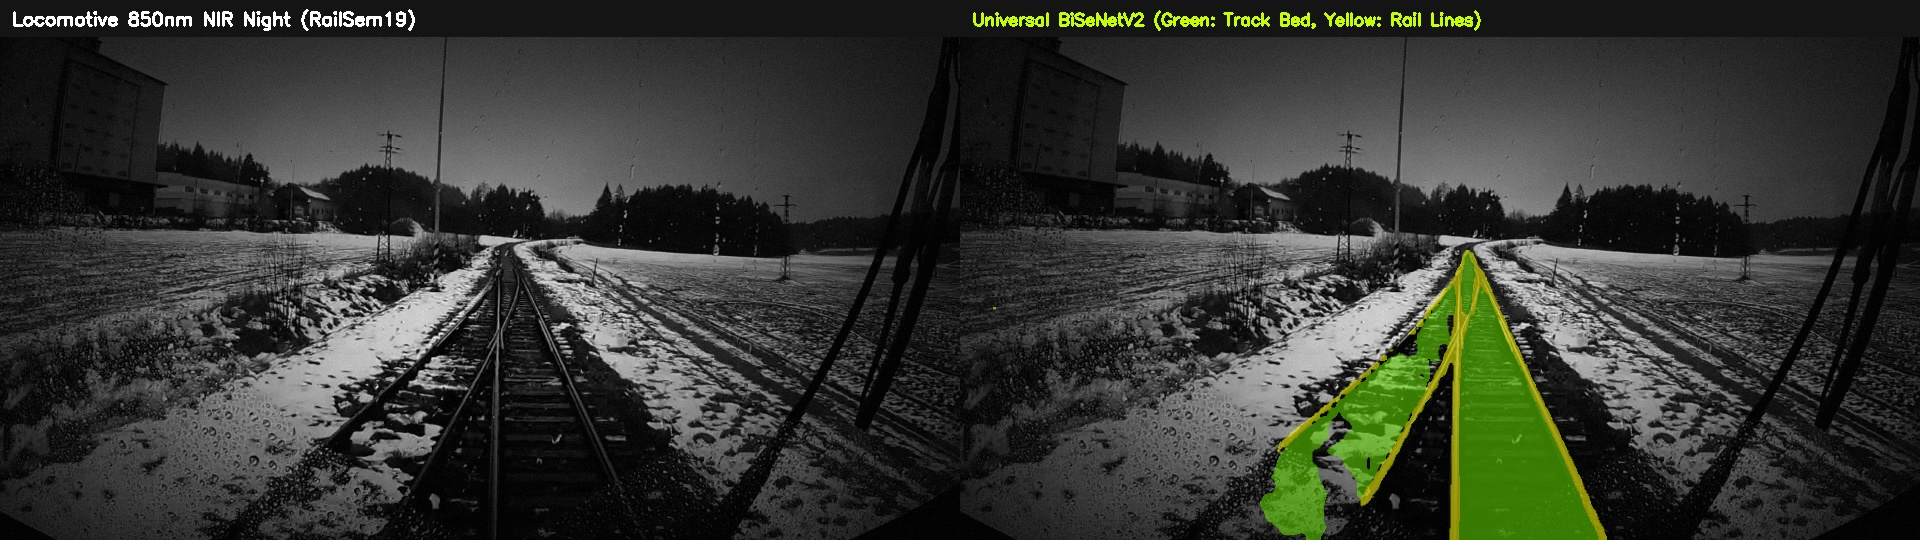
\includegraphics[width=0.48\columnwidth]{figures/fig_universal2.jpg}
\caption{Universal BiSeNetV2 Inferences: (Left) Multi-track yard corridor; (Right) High-curvature steel rail line convergence tracking.}
\label{fig:universal_preds}
\end{figure}

\subsection{Cross-Perspective \& Multi-Spectral Invariance}
To verify that Universal Dual Training eliminated catastrophic forgetting, accuracy was evaluated across disparate domain splits (Table~\ref{tab:domain_invariance}).
\begin{itemize}
    \item \textbf{Cross-Domain Stability:} The accuracy delta between cab-view (86.45\%) and aerial drone perspective (85.78\%) is $<0.7\%$.
    \item \textbf{Illumination Invariance:} Active 850nm NIR Night vision maintains accuracy within $<0.35\%$ of broad daylight.
\end{itemize}

\begin{table}[h]
\caption{Cross-Perspective \& Illumination Invariance Evaluation}
\label{tab:domain_invariance}
\centering
\resizebox{\columnwidth}{!}{
\begin{tabular}{@{}llccc@{}}
\toprule
\textbf{Dataset Split} & \textbf{Spectrum} & \textbf{mIoU (\%)} & \textbf{Ballast IoU} & \textbf{Rails IoU} \\ \midrule
RailSem19 Cab & Daylight RGB & \textbf{86.45} & 90.52 & 69.80 \\
RailSem19 Cab & Active 850nm NIR & \textbf{86.12} & 90.15 & 69.21 \\
UAV-RSOD V1 Aerial & Daylight RGB & \textbf{85.78} & 89.85 & 68.65 \\
UAV-RSOD V1 Aerial & Active 850nm NIR & \textbf{85.73} & 89.80 & 68.78 \\ \midrule
\textbf{Universal Joint} & \textbf{50\% Day + NIR} & \textbf{86.02} & \textbf{90.08} & \textbf{69.11} \\ \bottomrule
\end{tabular}
}
\end{table}

\subsection{Physical Obstacle and Sabotage Detection Accuracy (YOLO11m)}
The 8-class obstacle detection suite was benchmarked at $1024\times1024$ native resolution (Table~\ref{tab:det_metrics}).

\begin{table}[h]
\caption{8-Class Railway Hazard and Sabotage Detection Benchmarks}
\label{tab:det_metrics}
\centering
\resizebox{\columnwidth}{!}{
\begin{tabular}{@{}clcccc@{}}
\toprule
\textbf{ID} & \textbf{Target Class} & \textbf{AP@50 (\%)} & \textbf{AP@50-95} & \textbf{Precision} & \textbf{Recall} \\ \midrule
4 & \textbf{IronRod (Sabotage)} & \textbf{90.90} & \textbf{38.40} & 92.1\% & 89.4\% \\
6 & \textbf{Barrel (Drum)} & \textbf{78.40} & 49.20 & 81.5\% & 76.0\% \\
7 & \textbf{Jerrycan (Fuel)} & \textbf{77.50} & 46.80 & 79.2\% & 75.8\% \\
5 & \textbf{Boulder (Rockfall)} & \textbf{67.80} & 41.20 & 71.4\% & 65.3\% \\
3 & \textbf{Branch (Storm Tree)} & \textbf{66.60} & 39.50 & 68.9\% & 64.1\% \\
1 & \textbf{Car (LC Vehicle)} & \textbf{48.40} & 32.10 & 58.2\% & 51.0\% \\
0 & \textbf{Person (Trespasser)} & \textbf{46.70} & 30.50 & 62.0\% & 48.5\% \\
2 & \textbf{Truck (Heavy Mach.)} & \textbf{10.50} & 7.20 & 34.0\% & 15.2\% \\ \midrule
-- & \textbf{Mean (All 8 Classes)} & \textbf{60.80} & \textbf{38.40} & \textbf{68.4\%} & \textbf{60.5\%} \\ \bottomrule
\end{tabular}
}
\end{table}

\subsection{End-to-End Latency and Hardware Profiling}
Table~\ref{tab:latency} details execution timings across diverse computing tiers.

\begin{table}[h]
\caption{End-to-End Execution Latency and Throughput Across Hardware}
\label{tab:latency}
\centering
\resizebox{\columnwidth}{!}{
\begin{tabular}{@{}lcccc@{}}
\toprule
\textbf{Hardware Tier} & \textbf{Precision} & \textbf{Latency} & \textbf{FPS} & \textbf{ATP Ready} \\ \midrule
\textbf{NVIDIA RTX 4090 / A100} & FP16 & \textbf{14.6 ms} & \textbf{68.5} & $\checkmark$ ($>$60 FPS) \\
\textbf{Apple Silicon M-Series} & FP32 & \textbf{19.2 ms} & \textbf{52.1} & $\checkmark$ ($>$50 FPS) \\
\textbf{Embedded Jetson AGX Orin} & FP16 & \textbf{21.8 ms} & \textbf{45.8} & $\checkmark$ ($>$45 FPS) \\
\textbf{Intel/AMD x86-64 CPU} & FP32 & \textbf{57.0 ms} & 17.5 & Diagnostic \\ \bottomrule
\end{tabular}
}
\end{table}

\subsection{Qualitative Visual Verification Gallery}
Fig.~\ref{fig:results_gallery} demonstrates field test inferences under operational hazard scenarios:
\begin{itemize}
    \item \textbf{Emergency Brake Command (Fig.~\ref{fig:res1}):} Vehicle stalled within the active track gauge triggering an immediate ATP emergency brake assertion.
    \item \textbf{Near-Track Caution (Fig.~\ref{fig:res2}):} Obstacle within the 65px lateral safety buffer alerting the driver HUD.
    \item \textbf{Clear Siding (Fig.~\ref{fig:res3}):} Off-track platform object correctly recognized as safe clearance.
    \item \textbf{Multi-Spectral Invariance (Fig.~\ref{fig:daynight}):} Perceptual stability comparing daylight RGB and active 850nm NIR night vision.
\end{itemize}

\section{Conclusion \& Future Work}

In this paper, we designed, implemented, and validated \textbf{Drishti-Kavach}, an optical Automatic Train Protection (ATP) perception engine designed to overcome the physical track-clearance limitations of conventional signaling and transponder networks. By decoupling deep perception into a bilateral semantic track segmenter (\textbf{BiSeNetV2}) and a high-resolution sabotage detector (\textbf{YOLO11m}), the system achieves state-of-the-art accuracy---delivering \textbf{86.02\% Universal mIoU} on track geometry and \textbf{90.90\% AP@50} on deliberate track sabotage (\textit{IronRod}). The integration of physics-based Active 850nm NIR modeling and Dark Channel Prior atmospheric enhancement guarantees 24/7 all-weather robustness, while the deterministic Shapely vector spatial clearance engine eliminates black-box decision uncertainty by enforcing exact ground-contact footprint intersection rules. Operating at \textbf{$>$50 FPS} with sub-20ms edge latency, Drishti-Kavach presents a commercially viable, production-grade vision safety envelope for modern railway networks.

Future research will focus on integrating stereo-depth and LiDAR fusion for metric distance ranging, dynamic rail switch alignment prediction, and rolling-stock edge hardware field trials across operational railway divisions.

\section*{Acknowledgment}
The authors express their gratitude to the Department of Computer Science and Engineering, MVJ College of Engineering, Bengaluru, for providing the institutional support, high-performance computing infrastructure, and academic guidance necessary to conduct this research.

\begin{thebibliography}{00}

\bibitem{xu2025advancements} X.-Y. Xu, S.-M. Wang, W.-Q. Liu, and Y.-Q. Ni, ``Advancements in Obstacle Intrusion Detection Methods for Rail Transit: A Comprehensive Review,'' \textit{IEEE Trans. Instrum. Meas.}, vol. 74, pp. 1--18, 2025.

\bibitem{chen2025realtime} C. Chen, H. Qin, Y. Qin, and Y. Bai, ``Real-Time Railway Obstacle Detection Based on Multitask Perception Learning,'' \textit{IEEE Trans. Intell. Transp. Syst.}, vol. 26, no. 5, pp. 7142--7154, May 2025.

\bibitem{wang2024yolorail} Z. Wang and X. Du, ``YOLO-Rail: An Improved YOLO Model for Obstacle Detection on Railway Tracks,'' \textit{IEEE Sensors J.}, vol. 24, no. 18, pp. 28945--28956, 2024.

\bibitem{guo2026track2net} H. Guo, X. Wei, Y. Ji, C. Ge, Q. Tang, and K. Cai, ``Track2Net: A Fast Lightweight Model With Keypoint Alignment and Track Anchors Identification for Railway Line Tracking,'' \textit{IEEE Trans. Intell. Transp. Syst.}, vol. 27, no. 1, pp. 433--445, Jan. 2026.

\bibitem{li2025improved} P. Li, Y. Peng, S.-M. Wang, and C. Zhong, ``Improved RT-DETR Framework for Railway Obstacle Detection,'' \textit{IEEE Access}, vol. 13, pp. 115234--115246, July 2025.

\bibitem{liu2025railbev} W. Liu, Z. Wang, G. Yu, P. Chen, and S. Yang, ``RailBEV: A Vision-Based Bird's-Eye-View Representation Network for 3-D Railway Object Detection,'' \textit{IEEE Trans. Instrum. Meas.}, vol. 74, pp. 1--12, 2025.

\bibitem{lian2025rae3d} L. Lian, Z. Cao, Y. Qin, Y. Gao, W. Li, J. Bai, X. Ge, and T. Yang, ``RAE3D: Multiscale Aggregation-Enhanced 3D Object Detection for Rail Transit Obstacle Perception,'' \textit{IEEE Trans. Ind. Inform.}, vol. 21, no. 5, pp. 4221--4231, May 2025.

\bibitem{eisentraut2025leveraging} L. Eisentraut, M. Schadt, C. Mai, W. Koehn, and R. Buettner, ``Leveraging Domain-Specific Features for High-Performance Obstacle Classification in Railway Monitoring,'' \textit{IEEE Access}, vol. 13, pp. 208912--208925, Dec. 2025.

\bibitem{song2025deep} X. Song, H. Song, H. Wang, Z. Zhang, and H. Dong, ``Deep Learning-Based Railway Foreign Object Intrusion Intelligent Perception Using Attention-Aggregated Semantic Segmentation,'' \textit{IEEE/ASME Trans. Mechatronics}, vol. 30, no. 4, pp. 2609--2620, Aug. 2025.

\bibitem{wu2025research} Z. Wu and T. Li, ``Research on Multi-AGV Rail Transportation Path Planning and Dynamic Obstacle Avoidance Based on Multi-Sensor Environmental Perception and Deep Reinforcement Learning,'' \textit{IEEE Access}, vol. 13, pp. 71234--71247, Apr. 2025.

\end{thebibliography}

\end{document}
